\documentclass[a4paper, 12pt]{article}

% Sprache
% \usepackage[ngerman]{babel}
\usepackage[english]{babel}

% Pakete
\usepackage[utf8]{inputenc}
\usepackage[T1]{fontenc}
\usepackage{amsmath}
\usepackage{amssymb}
\usepackage{geometry}
\usepackage{fancyhdr}
\usepackage{graphicx}
\usepackage{hyperref}
\usepackage{titlesec}
\usepackage{booktabs}
\usepackage{framed} 
\usepackage{array}

\setlength{\parindent}{0pt}
\geometry{a4paper, margin=1in, headsep=35pt}
\titlespacing*{\subsection}{0pt}{*1}{1\baselineskip}
\setlength{\skip\footins}{1\baselineskip}

% Referenzen
\usepackage{csquotes}
\usepackage[style=verbose-ibid,backend=bibtex]{biblatex}

% Kopfzeile anpassen
\pagestyle{fancy}
\fancyhead{}
\fancyhead[L]{\veranstaltung \\ Projekt: \blatt}
\fancyhead[C]{\textbf{Jan-Niclas Loosen}\\ \textbf{Mat.Nr. 1540907}}
\fancyhead[R]{Universität Trier\\ \today}

% Variablen für Anpassungen
\newcommand{\blatt}{Report} % Nummer des Übungsblatts
\newcommand{\veranstaltung}{Softwaretechnik II} % Name der Veranstaltung
\bibliography{references.bib} % Name der BibTex-Datei

\begin{document}
	
\subsection*{The Smell of Stars -- A small study on the correlation between GitHub popularity and code quality.}

GitHub is an online platform for the management of source code and provides collaborative tools for joint development. Meanwhile, it has become the central management and storage location for a large number of open source projects. A key element of the social platform is the “Star” function, which allows users to favorite projects.\\

A study by Hudson Borges and Marco Tulio Valente\autocite{Borges2018} suggests that the awarding of stars has a distinct social media character. According to their study, the star function is used in particular to bookmark interesting projects or to express appreciation. Borges and Valente further determined that the number of stars correlates moderately with an increased number of contributors.\\

A higher number of contributors favors the assumption that a high number of stars can be an indicator of high-quality software solutions. The purpose of this small study is to systematically investigate a possible correlation between the popularity of open source projects -- measured by the number of stars -- and the quality of the source code.\\
	
\subsection*{Study Design}

Software quality can be examined on a variety of dimensions. Two of these are the number of \textit{bad smells} and the \textit{cognitive complexity}\autocite{Bogner2022}, which are both easy to measure. Bad smells are patterns that indicate problematic code passages, structural defects or high-maintenance areas. Cognitive complexity, on the other hand, measures how challenging it is for developers to understand and maintain the code based on the complexity of control structures and logical branches. Both metrics can be acquired by static code analysis using the Community Edition of the \textit{SonarQube} software tool\autocite{SonarQube}. Since both values increase with the size of projects, these can be further normalized based on the \textit{non-comment lines of code} (NCLOC). By doing so, projects of different sizes can also be compared.\\

In order to prevent a bias effect created by the choice of programming language, repositories written in Ruby, PHP, JavaScript (JS) and Python were examined. Since these scripting languages do not require a compilation step, they are much easier to evaluate with SonarQube. Although 960 repositories were originally planned, the automatic analysis of particularly large repositories led to timeouts and problems with limited memory, so that the final sample comprises 899 repositories. A detailed overview of the crawled repositories can be found in Table \ref{tab:repo_counts}. All projects were crawled using the GitHub API\autocite{GitHub-Api}, whereby the selection was not random but based on the best match pattern. This approach selected the best matching repositories for the applied search parameters.

\begin{table}[ht]
\centering
\begin{tabular}{|c|c|c|c|c|c|c|}
\hline
\textbf{Category} & \textbf{Stars} & \textbf{JS} & \textbf{PHP} & \textbf{Python} & \textbf{Ruby} & \textbf{Total} \\
\hline
Popular & $40 < x < 400$ & 110 & 110 & 108 & 114 & 457\\
\hline
Usual & $ 4000 < x $ & 116 & 112 & 113 & 116 & 442 \\
\hline
\end{tabular}
\caption{Overview of the automatically crawled projects.}
\label{tab:repo_counts}
\end{table}

In accordance with the research question, it was further necessary to decide which repositories should be categorized as popular or usual. In this study, repositories with more than 4000 stars were categorized as popular, while repositories with less than 400 stars were considered to be common. Early analyses revealed that without a lower limit, several empty repositories were included in the dataset. A minimum number of 40 stars was introduced as an additional criterion to prevent this. The disjoint groupings combined with the normalized results allow the application of the \textit{Mann-Whitney U-test} and \textit{Cohans-D} to statistically evaluate the differences between the crawled probesets.\\

The initial assumption of this study is that popular repositories indeed have a higher code quality compared to ordinary repositories. Considering the previous categorization, the following null and alternative hypotheses can be formulated:

\begin{table}[ht]
\centering
\renewcommand{\arraystretch}{1.4}
\begin{tabular}{p{0.45\linewidth} p{0.45\linewidth}}
\textbf{Null Hypotheses} & \textbf{Alternative Hypotheses} \\
\specialrule{2pt}{0pt}{0pt} 
$\mathbf{A_0}$: There is no significant difference in the number of code smells between popular repositories and usual repositories. 
& $\mathbf{A_1}$: Popular repositories tend to exhibit fewer code smells compared to usual repositories. \\[1ex]
$\mathbf{B_0}$: There is no significant difference in the cognitive complexity between popular repositories and usual repositories.
& $\mathbf{B_1}$: Popular repositories tend to have a lower cognitive complexity compared to usual repositories. \\
\end{tabular}
\end{table}

The assessments in this study were carried out using two Python scripts, one responsible for crawling and the other for analysis. Both scripts are available in the GitHub repository associated with this report at \href{https://github.com/jnloos/The-Smell-of-Stars}{https://github.com/jnloos/The-Smell-of-Stars}. In addition to the required Python libraries, a locally accessible instance of the SonarQube Community Server (e.g. in a running Docker container) is required to execute the code. The SonarQube CLI must also be installed and stored in the system's path variables.\\

\subsection*{Evaluation}

The descriptive analysis of the normalized results showed that the repositories with less than 400 stars have a slightly higher number of bad smells than the popular ones. Specifically, the common group has a mean of 0.03038 and a median of 0.01708 and popular repositories have a mean of 0.02429 and a median of 0.01501. The scatter indicated by the standard deviations 0.03602 for common repositories and 0.02831 for popular repositories and the observed maximum values of 0.224327 and 0.198731 indicate that although most repositories in both groups have a relatively low number of bad smells per NCLOC while a moderate dispersion is present. Figure \ref{fig:box-smells} shows a boxplot that visually compares the distribution of bad smells in the two groups.\\

\begin{figure}[h]
  \centering
  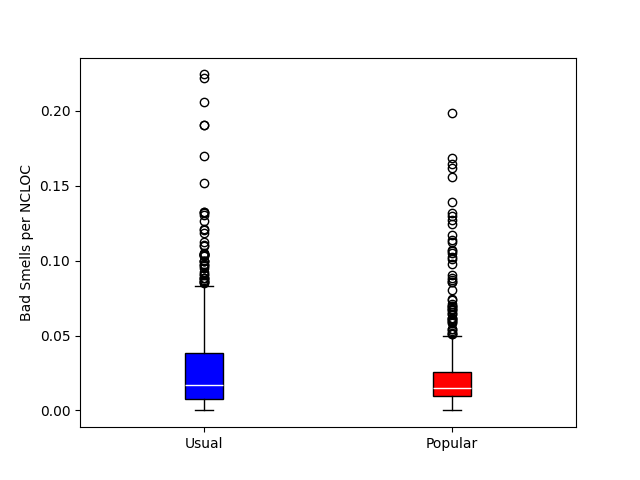
\includegraphics[width=0.85\textwidth]{../media/smells-boxplot.png}
  \caption{Boxplot comparing the number of bad smells per NCLOC in usual (40--400 stars) and popular GitHub repositories (>4000 stars).}
  \label{fig:box-smells}
\end{figure}

Nevertheless, both the Mann-Whitney U-test and Cohen's d ($U = 104901.0$, $p \approx 0.316$) effect size suggest that the differences in bad smells between the common and popular repositories are not statistically significant. The observed differences could therefore be attributed to random variation rather than a true statistical effect in, despite a tendency for slightly fewer bad smells in popular repositories.

\vspace{0.5em}
\begin{leftbar}
The results show a slight tendency that repositories with more than 4000 stars tend to have fewer bad smells than usual projects. However, the overall difference is not sufficient for statistical significance so that hypothesis $\mathbf{A_0}$ must be accepted.
\end{leftbar}
\vspace{0.5em}

Furthermore, the by the NCLOC normalized cognitive complexity of common repositories can be described by a mean value of 0.12823 and a median of 0.09091. With a mean value of 0.11331 and a median of 0.08412, popular projects again appear to be marginally less complex. The values have a standard deviation of 0.11643 for common and 0.10408 for popular repositories, which means that the scatter around the respective mean values is quite similar. The boxplot in Figure \ref{fig:box-cmplx} illustrates these observations once again.\\

The Mann-Whitney U-test ($U = 103923.5$, $p \approx 0.452$) and the corresponding Cohen's d effect size show no statistically significant differences between the groups in the inferential analysis. Similar to the Bad Smells per NCLOC, this emphasizes the observation that popular repositories appear to have a slightly lower cognitive complexity on average. However, the statistical significance is even smaller then the differences of the bad smells.

\begin{figure}[h]
  \centering
  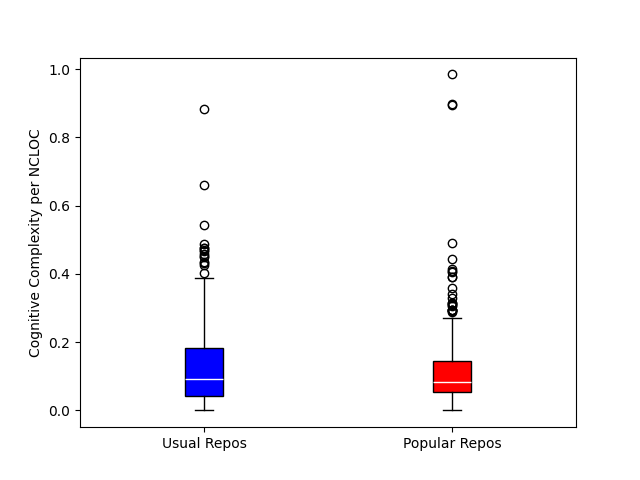
\includegraphics[width=0.85\textwidth]{../media/cmplx-boxplot.png}
  \caption{Boxplot comparing the determined cognitive complexity per NCLOC of usual (40--400 stars) and popular GitHub repositories (>4000 stars).}
  \label{fig:box-cmplx}
\end{figure}

\vspace{0.5em}
\begin{leftbar}
The statistical differences in terms of the normalized cognitive complexity are insignificant. In consequence, the null hypothesis $\mathbf{B_0}$ must be accepted. 
\end{leftbar}
\vspace{0.5em}

An interesting finding emerges when only Python, JavaScript and PHP repositories are examined and Ruby is excluded. With the smaller sample collection, the statistically analysis provided $U = 62540.0$ and $p \approx 0.0081$ for the number of bad smells as well as $U = 62222.5$ and $p \approx 0.0117$ for the cognitive complexity per NCLOC. These results indicate that popular repositories in these languages have statistically significantly fewer bad smells and lower cognitive complexity than their less popular countersamples.\\

This statistical significance vanishes as soon as Ruby repositories are equally included in the analysis. The reason for this is that a deviating pattern can be observed in Ruby repositories: Here, unlike in the other languages, popular repositories tend to have a higher number of bad smells as well as a higher complexity. This considerably counteracts the trend that has been observed for the other programming languages.\\

These observations suggest that the quality differences between popular and unpopular repositories could depend heavily on the considered programming languages. It therefore seems worthwhile to investigate the language-specific characteristics in greater depth as part of further quantitative studies. Figures \ref{fig:scatter-smells} and \ref{fig:scatter-smells-ruby} are available on the next page and exemplarily illustrate the contradictory trends for the bad smells for PHP and Ruby.\\

\begin{figure}[h!]
  \centering
  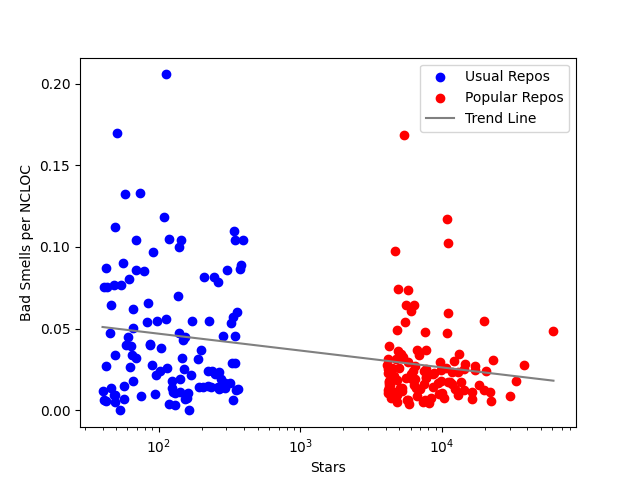
\includegraphics[width=0.85\textwidth]{../media/php-smells-scatterplot.png}
  \caption{Scatterplot showing the relationship between repository stars and bad smells per NCLOC in the evaluated PHP repositories. The trend line was fitted using regression.}
  \label{fig:scatter-smells}
\end{figure}

\begin{figure}[h!]
  \centering
  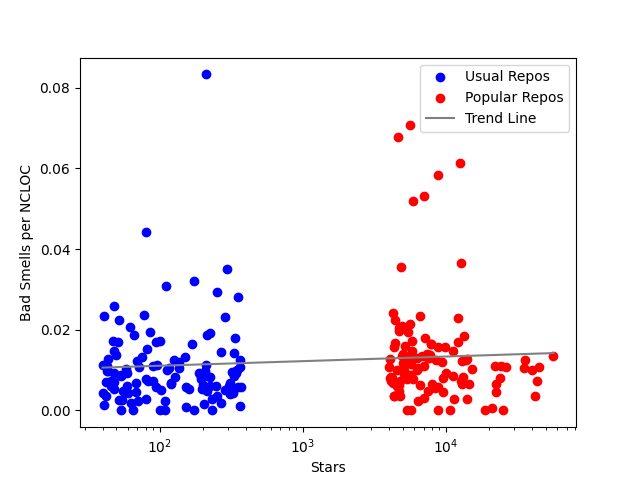
\includegraphics[width=0.85\textwidth]{../media/ruby-smells-scatterplot.png}
  \caption{Scatterplot showing the relationship between repository stars and bad smells per NCLOC in the evaluated Ruby repositories. The trend line was fitted using regression.}
  \label{fig:scatter-smells-ruby}
\end{figure}

\subsection*{Threads to Validity}

Due to the short time frame for the data collection, it was only possible to analyze 899 projects. In particular the analysis with SonarQube was both time- and resource-intensive. According to the experience gained, the examination of a single repository required 5--15 minutes on average. The technical limitations of the utilized computer (32 GB RAM) furthermore limited the parallel execution to 2 simultaneously running threads.  Consequently, only a small fraction of the available free GitHub projects were examined, meaning that a bias effect cannot be ruled out. The observations regarding Ruby should be treated with particular caution, as they are based on only 230 samples.\\

Another important aspect is that the quality of software projects is a versatile concept and involves much more than just capturing bad smells and cognitive complexity. Criteria such as documentation, test coverage, maintainability and usability are also crucial for a comprehensive assessment of software quality. In order to obtain a complete picture of the quality of projects, these other dimensions must also be included in future studies.\\

\subsection*{Conclusion}
This study compared popular GitHub repositories (>4000 stars) with less popular ones (40-400 stars) to investigate whether popularity is related to better code quality. The comparison was based on the number of bad smells and the cognitive complexity per NCLOC from a total of 899 public projects. Although a slight tendency emerged for popular repositories to have slightly better quality metrics, the differences across the entire samples were not statistically significant. This result is surprising, as this report originally assumed that the quality of code is superior in popular repositories. Nevertheless, a selective analysis revealed that the quality of Python, JavaScript and PHP repositories actually improves statistically significantly with increasing popularity. For Ruby repositories, on the other hand, a strong opposite trend can be observed that offsets the significance in the overall analysis.\\

From a practical perspective, these results suggest that developers and project maintainers should be cautious when using GitHub stars as an indicator of code quality. While popularity can indicate community approval and visibility, it is not necessarily a guarantee of high code quality in all languages. Thus, a deeper and language-specific assessment is crucial for making informed decisions in project selection and development strategies.\\

The observed differences between the programming languages are particularly worthwhile for further investigation. Such research should address the limitations identified in this work by considering more samples and including additional dimensions of software quality. If the codes associated with this study will be reused, it is highly recommended to use a more powerful computer for the evaluation process.\\
	
\end{document}
